\documentclass{article}

\setlength{\paperwidth}{210mm}
\setlength{\paperheight}{297mm}
\setlength{\hoffset}{-12mm}
\setlength{\voffset}{-10mm}
\setlength{\evensidemargin}{0mm}
\setlength{\oddsidemargin}{0mm}
\setlength{\topmargin}{0mm}
\setlength{\headheight}{0mm}
\setlength{\headsep}{5mm}
\setlength{\textheight}{256.2mm}
\setlength{\textwidth}{184.2mm}
\setlength{\marginparsep}{0mm}
\setlength{\marginparwidth}{0mm}
\setlength{\footskip}{5mm}
\setlength{\marginparpush}{0mm}


\usepackage[spanish]{babel}
\usepackage[utf8]{inputenc}
\usepackage{graphicx}

\pagestyle{myheadings}
\markright{IA - Práctica de búsqueda local}

\title{\Huge{Práctica de búsqueda local} \\
\vspace{15mm}
   \Large{Laboratorio de Inteligencia Artificial}}
\author{Marion Not - Michael Boris Mandirola}
\date{Primavera 2010-2011}

\begin{document}

\maketitle

\newpage

\tableofcontents

\newpage

\section*{Introducción}

El objetivo de esta práctica es analizar y resolver un problema de optimización
logística mediante algoritmos de búsqueda local. Definiremos la representación
del problema como estado y estudiaremos la influencia de los elementos que
intervienen en esta búsqueda y que hemos visto a clase (estado inicial, función
heurística y operadores) bajo diferentes condiciones sobre los parámetros del
problema.

Usaremos dos tipos de algoritmos de búsqueda local : el Hill Climbing y el
Simulated Annealing. Como el objetivo de la práctica no es la implementación de
estos algoritmos, usaremos las herramientas proporcionadas por el package AIMA. 
En el caso del Simulated Annealing, también estudiaremos la influencia de los 
parámetros del algoritmo.

\section{Representación del problema}

El contexto del problema es el siguiente : Una empresa de transporte está
contratada por una compañía para gestionar el encaminamiento de productos desde
un almacén central hasta unos centros de producción.

Cada día, los centros realizan un conjunto de peticiones de diferentes tipos y 
cantidades de productos que se tienen que entregar a una cierta hora. El pago se
realiza en función de la cantidad de productos entregados y la puntualidad con
la cual han llegado al centro.

La empresa de transporte quiere optimizar estas entregas, sabiendo que manda un
transporte a cada centro en cada hora en punto del día.
No tenemos que gestionar la recogida de productos en el almacén, ni el recorrido
de los transportes, ni la cantidad de camiones físicos que se necesitan :
Suponemos que la empresa dispone de una flota suficiente para hacer todas las
entregas en tiempo.
Solucionaremos este problema para un solo día, pues las peticiones no entregadas
no estarán desplazadas al día siguiente.

\subsection{Identificación de los elementos relevantes}

Para cada problema, tendremos unos elementos constantes, unos elementos
específicos del problema y unos elementos variables que se tendrán que
determinar para llegar a la solución.

\subsubsection{Constantes}

\begin{description}
\item[Centros de producción :] Como lo hemos dicho, el número de centros esta 
fijado a 6.
\item[Horas de entrega :] Las entregas se harán a cada hora en punto del día. La
primera se hará a las 8 y la última a las 17, para un total de 10 horas de
entrega.
\item[Transportes :] Tendremos un transporte para cada hora del día y cada
centro, es decir 60 transportes en total. La capacidad de los camiones usados
sera de 500, 1000 o 2000kgs, en proporción variable.
\item[Peticiones :] Las peticiones se harán para una de las horas de entregas y
para una cantidad de productos de 100, 200, 300, 400 o 500kgs.
\end{description}

\subsubsection{Elementos específicos del problema}

\begin{description}
\item[Peticiones :] Todas las peticiones estarán generadas al principio de la
resolución mediante unos parámetros especificados por el usuario. Por lo tanto,
serán diferentes para cada problema. Se tendrán que especificar :
\begin{itemize}
\item El número de peticiones
\item La distribución de probabilidad de cantidad de productos de las entregas
\item La distribución de probabilidad de horas de entrega
\end{itemize}
Las peticiones estarán repartidas de forma equiprobable entre los centros.
El tipo de producto pedido no tienen ninguna influencia.
\item[Transportes :] Se tendrá que especificar la distribución de probabilidad
de capacidades de los transportes, es decir cuantos de los 60 transportes
tendrán una capacidad de 500kgs, cuantos de 1000 y cuantos de 2000.
\item[Parámetros de la búsqueda :] Se precisará que tipo de estado inicial,
algoritmo de búsqueda y función heurística se tienen que usar. 
\end{description}

\subsubsection{Elementos de la solución}

Para llegar a la solución, se tendrán que determinar :
\begin{itemize}
\item La repartición de los 60 transportes, es decir que capacidad de transporte
se asignará a cada hora de cada centro.
\item La repartición de las peticiones en los transportes. El orden de las
peticiones en el transporte no importa.
\end{itemize}

\subsection{Definición del Estado}

Hemos escogido una representación en acuerdo con la descripción del problema de
la parte anterior.

\subsubsection{Implementación}

\begin{center}
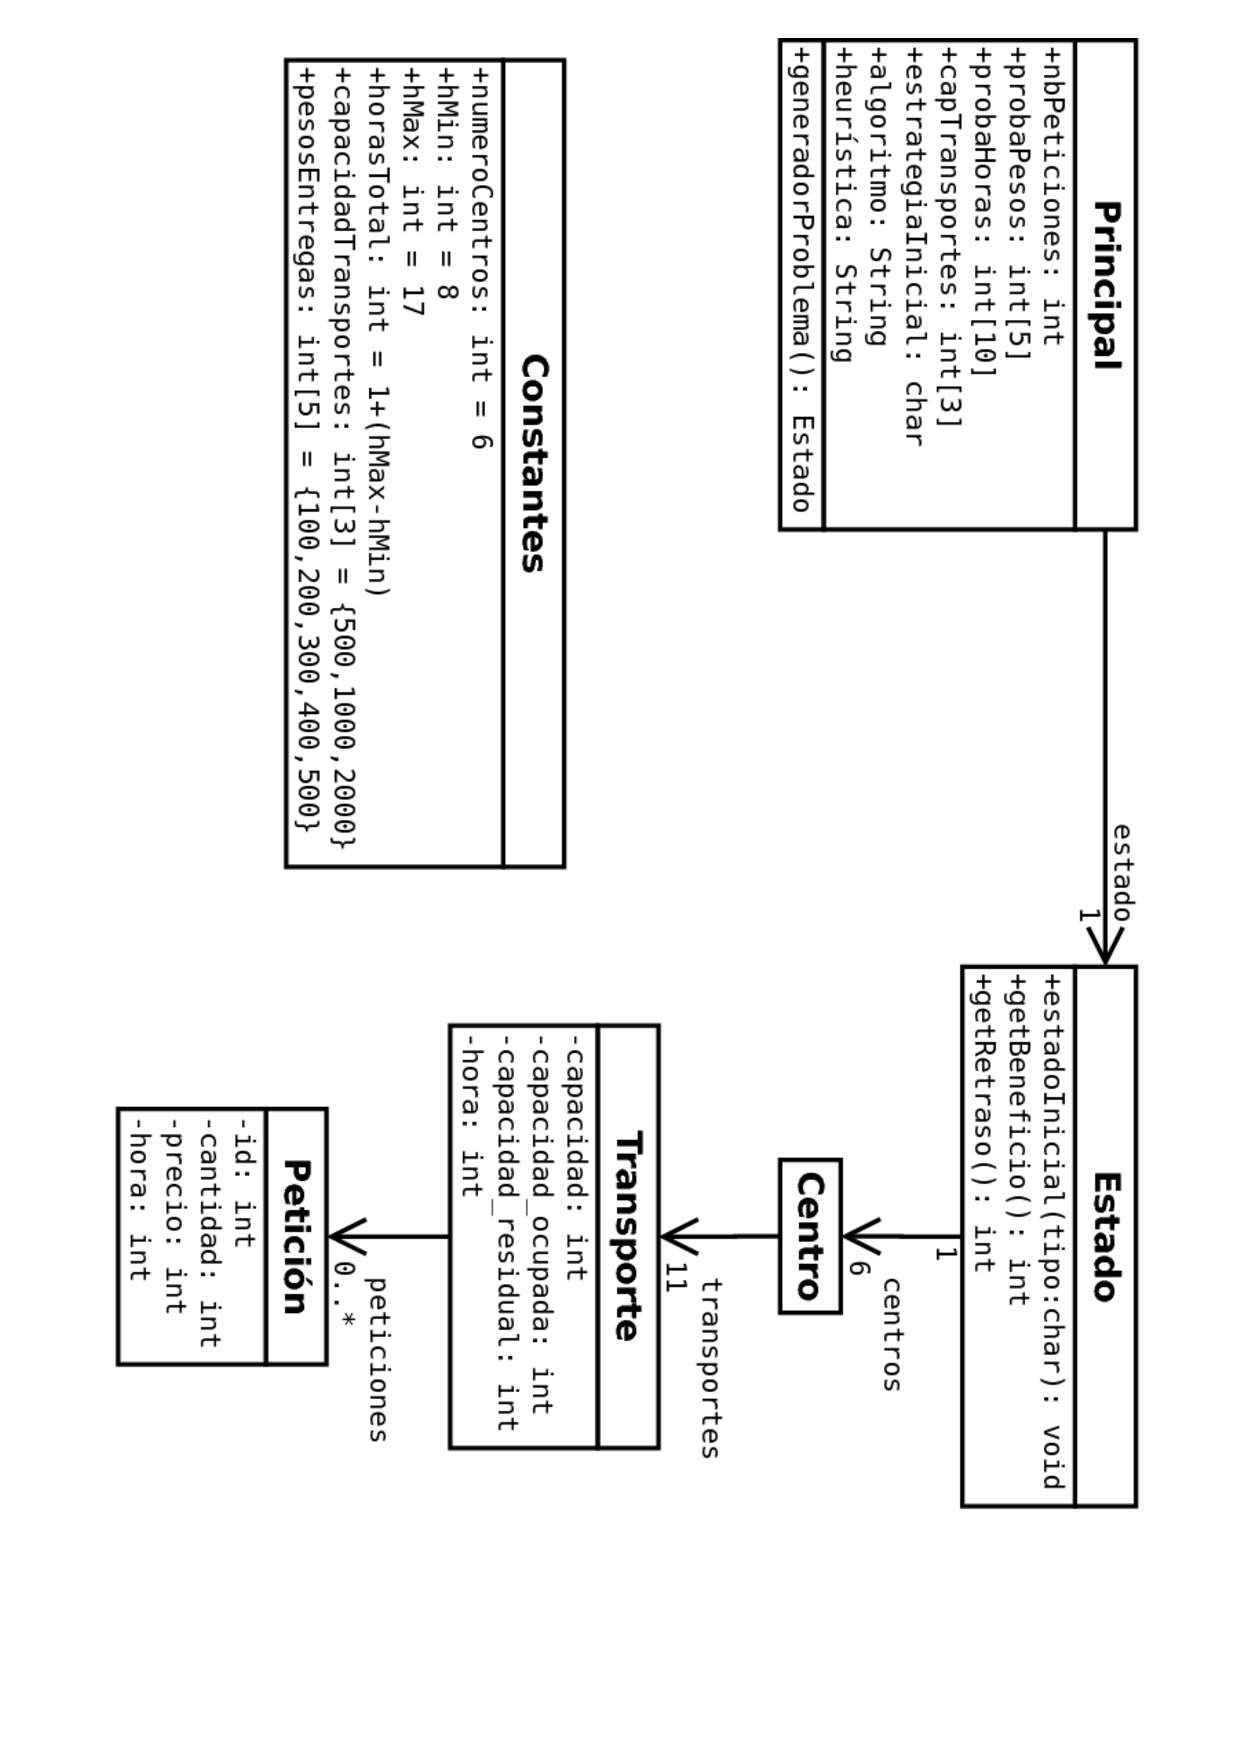
\includegraphics[width=14cm, angle=90]{clases}\\
{\it Fig. 1.1 : Diagrama de clases de representación del problema.} 
\end{center}

\begin{itemize}
\item Una clase singleton Constantes contiene los elementos comunes a todos los
problemas.
\item Los elementos específicos serán leídos desde un fichero .txt y usados por
el Principal para generar un problema dado, es decir un conjunto de instancias
de la clase Petición y un Estado ``vacío'', donde las peticiones estarán
repartidas entre las 6 instancias de clase Centro pero no entregadas. Se crearán
11 instancias de clase Transporte : una para cada hora del día y una para
guardar las peticiones no entregadas.
\item A continuación, se generará el estado inicial de la búsqueda, es decir que
se atribuirá una capacidad a cada unos de los 60 transportes que corresponden a
una hora (los Transporte de peticiones no entregadas tendrán capacidad máxima) y
se repartirán las peticiones según la estrategia especificada.
\item Durante la resolución del problema, las peticiones se desplazarán de un
Transporte a otro, dentro del mismo Centro. También se podrá modificar la
repartición de las capacidades entre todos los 60 transportes. Ver la sección
siguiente para detalles sobre los operadores.
\end{itemize}

\subsubsection{Tamaño del espacio de búsqueda}

Si tenemos $N$ peticiones, repartidas igualmente entre 6 centros ($\frac{N}{6}$
peticiones/centro), que se pueden afectar a cualquier de los $10+1$ transportes,
contamos con $O(11^N)$ configuraciones posibles para la repartición de las
peticiones.

Si añadimos que cada uno de los 60 transportes puede tener una de 3 capacidades,
es decir $O(3^{60})$ configuraciones posibles, tenemos \textbf{un total de
$O(11^N*3^{60})$ estados posibles}.

Se tiene que tener en cuenta que en verdad, la suma de pesos de las peticiones
afectadas a un transporte no puede exceder su capacidad, y que tenemos un número
limitado de transportes de cada capacidad : Eso reduce el tamaño del espacio de
búsqueda.

Este tamaño es bastante importante, pero considerando que hacemos una búsqueda
local y que recorreremos solo una fracción del espacio, no es excesivo.

\subsection{Operadores}

\noindent Hemos implementado tres operadores diferentes :
\begin{enumerate}
\item Desplazamiento de una petición
\item Intercambio de capacidades de camiones
\item Intercambio de dos peticiones
\end{enumerate}

\subsubsection{Op1 : Desplazamiento de una petición}

\begin{description}
\item[Descripción :] Este operador desplaza una petición de un transporte a
otro transporte del mismo centro (ya que la asignación de una petición a un
centro no es cambiable). Está implementado para que sea posible desplazar una
petición desde o hasta el grupo de peticiones no entregadas, pero no desde un
transporte hasta sí mismo.
\item[Efecto :] Se disfruta de los ``huecos'' que pueden existir o crearse
dentro de los transportes, por ejemplo después de un cambio de capacidad de
camiones, para entregar peticiones no entregadas o entregadas con retraso.
\item[Condición de aplicación :] Este operador se puede aplicar sólo si la
hora de destino tiene una capacidad disponible suficiente para añadir la
petición.
\item[Factor de ramificación :] Para un conjunto de $N$ peticiones, el factor de
ramificación de este operador es de $O(10N)$, ya que cada petición se puede
desplazar a las 10 otras horas de su centro. Es linear, y debemos tener en
cuenta que la mayor parte de los desplazamientos no cumplirán la condición de
aplicación.
\item[Justificación de la elección :]
Hemos decidido implementar este operador porque es lo más evidente y lo más 
simple para desplazar peticiones, con un coste linear.
\item[Variante :] Una variante de este operador sería prohibir el desplazamiento
de peticiones hasta el grupo de no entregadas. El factor de ramificación pasaría
a ser $O(9N)$, y en práctica se eliminaría la generación de muchos sucesores,
ya que mover la petición hasta las no entregadas es el único movimiento que
siempre cumple la condición de aplicación. Además, estos estados no pueden ser
escogidos por el Hill Climbing porqué su heurística siempre es peor.

Sin embargo, decidir de no entregar una petición puede ser una decisión útil en
el caso del Simulated Annealing, ya que permite la evolución de más estados.
Entonces, hemos decidido guardar la primera versión del operador.
\end{description}

\subsubsection{Op2 : Intercambio de capacidades de camiones}

\begin{description}
\item[Descripción :] Este operador intercambia las capacidades de dos
transportes, que pueden ser de dos centros diferentes. Sólo se cambia el valor
de la capacidad, no se intercambian las instancias de Transporte (y por lo
tanto, las peticiones). Así, se conserva la proporción de transportes de cada
capacidad. 

Sin embargo, el intercambio de camiones solo no cambia ninguna heurística. Por
eso, hemos decidido combinarlo con el desplazamiento de una petición : Se
intenta desplazar una petición no entregada al transporte que ha aumentado su
capacidad ; si no es posible, se escoge una petición entre las que se entregan
más tarde.

El operador está implementado para que no se puedan intercambiar dos camiones
que tengan la misma capacidad, y por supuesto que no se pueda cambiar la
capacidad máxima del transporte correspondiente a las peticiones no entregadas.
\item[Efecto :] Permite cambiar la capacidad total disponible en un centro o
repartir-la de forma diferente entre las horas. Así, se podría poner más
capacidad en centros que tienen una cantidad de peticiones más grande, o en las
horas más tempranas del día para reducir el retraso.
\item[Condición de aplicación :] Este operador se puede aplicar sólo si la
capacidad ocupada de cada transporte es inferior su nueva capacidad. 
\item[Factor de ramificación :] Cada transporte puede intercambiar su capacidad
con una diferente. Si tenemos una repartición de capacidades $\{C1,C2,C3\}$, el
factor de ramificación es $(C2+C3)^{C1}*(C3+C1)^{C2}*(C1+C2)^{C3} = 40^{60}$ si
tenemos una repartición equiprobable. Es constante y considerablemente más
pequeño en práctica.
\item[Justificación de la elección :] Intercambiar dos capacidades es la única
forma de manipular este parámetro sin cambiar la repartición de valores, ya que
tenemos 60 cantidades para 60 transportes. El desplazamiento de petición lo
realizamos considerando el uso primero de este operador, que es liberar
capacidad para entregar peticiones no entregadas o retrasadas.
\end{description}

\subsubsection{Op3 : Intercambio de dos peticiones}

\begin{description}
\item[Descripción :] Este operador intercambia dos peticiones del mismo centro,
pero de dos horas diferentes. Se puede hacer el intercambio con una petición no
entregada y también se pueden intercambiar dos peticiones de mismo peso.
\item[Efecto :] Permite realizar desplazamientos de peticiones que no se
conseguirían con los operadores precedentes, por ejemplo intercambiar una
petición adelantada con una retrasada. 
\item[Condición de aplicación :] Este operador se puede aplicar sólo si los
transportes tienen capacidad suficiente. Específicamente, si las peticiones no
tienen el mismo peso, el transporte de la más pequeña debe tener bastante
capacidad residual para contener la diferencia de pesos.
\item[Factor de ramificación :] Cada petición se puede intercambiar con todas
las otras peticiones del centro, con $N$ peticiones el factor de ramificación es
$N^{\frac{N}{6}}$, considerablemente mas elevado que para los dos previos
operadores.
\item[Justificación de la elección :] Hemos decidido implementar este algoritmo
al ver el porcentaje de estados que no mejoraban : Ofreciendo mas posibilidades
de evolución de los estados, esperemos obtener una mejoría consecuente de la
solución a pesar del factor de ramificación elevado.
\end{description}

\subsection{Funciones Heurísticas}

\subsubsection{Maximización del beneficio}

\begin{description}
\item[Definición de la variable evaluada :]
Para cada petición, la compañía pagará a la empresa de transporte un importe
basado sobre el precio base de las peticiones, indicado en la tabla 1.1. Este
precio depende únicamente de la cantidad de productos pedida, y la puntualidad
de la entrega.
\begin{center}
\begin{tabular}{|l|l|}
\hline
Peso & Precio\\
\hline
100 y 200kg & {\it peso} euros\\
300 y 400kg & 1,5x{\it peso} euros\\
500kg & 2x{\it peso} euros\\
\hline
\end{tabular}\\
{\it Tabla 1.1 : Precio base de las entregas.}
\end{center}

El importe pagado para cada petición entregada será el precio base menos unos
20\% del mismo para cada hora de retraso, es decir que para mas de 5h de retraso
le tocara pagar a la empresa de transporte.

Si una petición no esta entregada en el día, la empresa de transporte tendrá que
pagar el precio base de la petición mas unos 20\% del mismo para cada hora hasta
las 17.

El beneficio es la suma del importe (positivo o negativo) de todas las
peticiones.\\

Ejemplo : Para cada peso de petición, en la tabla 1.2 se indican los
importes correspondientes a una entrega en tiempo, una entrega con 1 y 7 horas
de retraso y no entrega, considerando que las peticiones se tenían que entregar
a las 10.
\begin{center}
\begin{tabular}{|l|l|l|l|l|l|l|}
\hline
Peso & En tiempo ($\leq$10h) & Retraso 1h (=11h) & Retraso 7h (=17h) & No
entregada\\
\hline
100kg & 100 & 80 & -40 & -240\\
200kg & 200 & 160 & -80 & -560\\
300kg & 450 & 360 & -180 & -1080\\
400kg & 600 & 480 & -240 & -1440\\
500kg & 1000 & 800 & -400 & -2800\\
\hline
\end{tabular}\\
{\it Tabla 1.2 : Ejemplos de importes.} \end{center}

\item[Contextualización :] La penalización para retraso y no entrega parece
realista en comparación con lo que esperaría una empresa en realidad. Sin
embargo, el hecho de que el beneficio no sea linear comparado con el peso y que
el tipo de producto no afecta corresponde seguramente a una simplificación del
problema, ya que en verdad los productos serian mas o menos caros y críticos
(mas penalización para retraso) y el peso tendría a disminuir para cantidades
mas grandes.
\end{description}

\subsubsection{Minimización del tiempo}

\begin{description}
\item[Definición de la variable evaluada :] Para esta heurística, consideraremos
para cada petición la diferencia \emph{absoluta} entre la hora de entrega
deseada y la hora de entrega efectiva. Pues, una petición entregada con
antelación afecta esta heurística de forma tan negativa como una petición
entregada con un retraso equivalente.

Si la petición no esta entregada en el día, consideraremos la diferencia entre
la hora de entrega deseada y las 8 del día siguiente. Por ejemplo : Una petición
que se debía entregar a las 10 y que no fue entregada tendra un ``retraso'' de
22h.

Sumaremos todas estas cantidades para obtener el valor de la heurística.
\item[Contextualización :] Esta heurística representa un otro aspecto de la
realidad de las empresas : Cuando se usa el método justo a tiempo, recibir
productos con antelación y tener que gestionar el stock implica también una
perdida de productividad, aunque en realidad una antelación de una hora no
tendría mucho impacto, y en general la antelación tendría menos efectos que el
retraso, que puede potencialmente paralizar la producción si el producto
transportado es crítico.

Ademas, se tendra que tenir en cuenta que un valor bueno del primer heuristica
no implica necesariamente un valor bueno del segundo.
\end{description}

\subsection{Estados Iniciales}

En un primer paso, hemos intentado generar estados diferentes con lógicas muy
distinctas, con la idea de buscar nuestros estados iniciales entre un grupo más
amplio y en particular elegir dos estados que tengan características diferentes
(tiempo de generación, complejidad del algoritmo, posibilidades de evolución,
calidad de la solución inicial).

Al final, hemos implementado cuatro tipos de estados iniciales que nos han
parecido interesantes :
\begin{enumerate}
\item ``Cuanto antes''
\item ``Por hora''
\item ``First-fit''
\item ``Vacío''
\end{enumerate}

\subsubsection{Ei1 : Cuanto antes}

\begin{description}
\item[Repartición de los camiones :] Se reparten las capacidades de transporte
de forma igual entre los centros, y se asignan los transportes con más capacidad
a las horas más tempranas.
\item[Repartición de las peticiones :] Las peticiones están entregadas cuanto
antes : Para cada centro, están ordenadas de forma ascendente por hora de
entrega, descendente por precio y asignadas a los transportes en orden,
empezando por el mas temprano que tenga capacidad residual.
\item[Calidad :] Este estado inicial no es muy costoso. Llega a una buena
solución, a veces óptima para la heurística de maximización del beneficio, pero
puede introducir mucha antelación y llevar a una solución mediocre para la
heurística de minimización del tiempo. Además, la repartición de los camiones
puede ser no óptima, por ejemplo si un centro se ve asignado una cantidad de
peticiones mas importante que otro.
\end{description}

\subsubsection{Ei2 : Por hora}

\begin{description}
\item[Implementación :] Las peticiones están ordenadas por precio y hora. Para
cada petición, se intenta entregarla en su hora de entrega con el algoritmo
siguiente :
\begin{enumerate}
\item Si no hay capacidad asignada al transporte, se asigna la capacidad mínima
disponible y se entrega la petición.
\item Si hay una capacidad libre suficiente, se entrega la petición.
\item Si hay una capacidad no suficiente y una capacidad más grande es
disponible , se asigna una capacidad mas grande y se entrega la petición.
\item Si no se puede asignar una capacidad más grande a la hora de entrega, se
intenta entregar la petición en la hora antes, siguiendo el mismo algoritmo.
\item Si se llega a las 8, se intenta entregar la petición en la hora siguiente,
siempre con el mismo algoritmo.
\item Finalmente, no se entrega la petición.
\end{enumerate}
Al final, si quedan transportes sin capacidad asignada, se asignan las
capacidades que quedan.
\item[Calidad :] Este algoritmo es mucho mas costoso, pero lleva a una solución
de calidad para ambos heurísticas.
\end{description}

\subsubsection{Ei3 : First-Fit}

\begin{description}
\item[Repartición de los camiones :] Los camiones se asignan como en el estado
``Cuanto antes''.
\item[Repartición de las peticiones :] Se recorren todas las peticiones (no
ordenadas), intentando entregarlas en su hora de entrega. Después,
iterativamente, se intentan entregar las peticiones no entregadas en las horas
más tempranas de la suya hasta las 8 y si no se tiene éxito, se intenta hacerlo
en las horas después hasta las 17.
\item[Calidad :] Similar al estado ``Cuanto antes'', este estado es más adaptado
a la heurística de minimización del tiempo.
\end{description}

\subsubsection{Ei4 : Vacío}

\begin{description}
\item[Repartición de los camiones :] Los camiones se asignan como en el estado
``Cuanto antes''.
\item[Repartición de las peticiones :] Las peticiones se quedan todas no
entregadas.
\item[Calidad :] Este estado es lo más barato, pero genera la peor solución
posible.
\end{description}

\newpage

\section{Experimentos}

\subsection{Implementación}

\subsubsection{Workflow de ejecución de pruebas}

El programa efectúa las pruebas sacando los parámetros necesarios de ficheros de
texto. Los ficheros están organizados en la siguiente manera :

\begin{itemize}
\item Linea 1 : Número de pruebas con estos parámetros - 1 Integer
\item Linea 2 : Número de peticiones - 1 Integer
\item Linea 3 : Distribución de capacidad de los camiones - 3 Integers para 500,
1000 y 2000kg - La suma de los 3 debe ser igual a 60.
\item Linea 4 : Distribución de pesos de las peticiones - 5 Floats para 100
hasta 500kg - La suma de los 5 debe ser igual a 1.
\item Linea 5 : Distribución de las horas de entrega - 10 Floats para 8h hasta
17h - La suma de los 10 debe ser igual a 1.
\item Linea 6 : Estrategia para generar el estado inicial - 1 Char
\item Linea 7 : Tipo de algoritmo - String - Puede ser "hc" o "sa".
\item Linea 8 : Tipo de heurística - String - Puede ser "gan" o "ret".
\end{itemize}

Cada experimento, pero, necesita una batería de pruebas con diferentes
parámetros. Así tenemos una carpeta para cada experimento con diferentes
ficheros para generar pruebas. Un {\it bash script} recibe en input el numero
del experimento y resuelve el problema con los ficheros de prueba pertinentes.

\subsubsection{Recuperación de resultados}

Para cada problema, son generados dos ficheros de salida, uno con el estado
inicial y el otro con el estado final. En estos ficheros tenemos:

\begin{itemize}
\item El valor de cada heurística
\item Los centros, y para cada centro :
	\begin{itemize}
		\item Cantidad de peticiones no entregadas
		\item Las horas y por cada hora de entrega
		\begin{itemize}		
			\item La capacidad total
			\item La capacidad ocupada
			\item La capacidad libre
			\item Las peticiones no entregadas y por cada petición		
			\begin{itemize}
			\item El identificador
			\item La hora de entrega supuesta
			\item La cantidad
			\item El precio
			\end{itemize}
		\end{itemize}
	\end{itemize}
\end{itemize}
También hay un fichero de estadísticas por cada experimento a que vamos
añadiendo datos sobre las pruebas. Este fichero está organizado como un CSV y
por cada prueba tenemos registrados:
\begin{itemize}
\item El numero de nodos desarrollados. 
\item El beneficio.
\item El porcentaje de mejoría de el beneficio.
\item El retraso
\item El porcentaje de mejoría de el retraso.
\item El tiempo de ejecución de la búsqueda.
\end{itemize}
Una linea vacía y una linea con el título del fichero de input dividen los diferentes grupos de pruebas (resultado de diferentes ejecuciones de el programa).

\subsection{Experimento 1 : Elección del conjunto de operadores}

\subsubsection{Contexto}

\begin{description}
\item[Elementos comparados :] Queremos elegir el conjunto de operadores que
vamos a usar en el resto de experimentos, entre los tres operadores que tenemos
implementados : \emph{Desplazamiento de petición (Op1), intercambio de camiones
(Op2) y intercambio de peticiones (Op3)}. Hemos decidido probar dos conjuntos :
\begin{enumerate}
\item Op1 + Op2
\item Op1 + Op2 + Op3
\end{enumerate}
Hemos decidido incluir imperativamente los operadores 1 y 2 en el conjunto, ya
que Op1 es el único operador que nos permite desplazar peticiones no entregadas
a las entregadas y Op2 es el único que mueve los camiones. Principalmente,
estudiaremos la influencia del operador Op3 sobre el tiempo de ejecución, la
bondad de la solución y el porcentaje de estados que mejoran.
\item[Número de pruebas :] 100 pruebas para cada conjunto de operadores.
\item[Estado inicial :] Hemos escogido el estado inicial ``Repartición por
hora'', que se puede mejorar bastante frecuentemente y no consume demasiado
tiempo.
\end{description}

\subsubsection{Resultados}

El porcentaje de mejoría del beneficio se calcula con la formula :
$\frac{ben. E_f - ben. E_i}{ben. E_f}$. Se ha calculado solo considerando los
estados mejorados, y luego en general.

\begin{center}
\begin{tabular}{|l|l|l|l|l|}
\hline
Conjunto & Estados mejorados & Beneficio &  \% de mejoría (global) & Tiempo de
ejecución (por iteración)\\
\hline
Op1 + Op2 & 5 & 97452 & 2,02\% (0,10\%) & 30,07ms (25,99ms)\\
\hline
Op1 + Op2 + Op3 & 16 & 97533 & 1,16\% (0,19\%) & 191,8ms (119,9ms)\\
\hline\\
\end{tabular}
{\it Tabla 2.1 : Resultados del experimento 1.}
\end{center}

\subsubsection{Conclusiones}

Como lo habiamos previsto, el operador Op3 provoca la evolución de mas estados.
Sin embargo, en media la solución hallada es menos buena. Ademas, el tiempo de
ejecución esta multiplicado por mas de 4.

Al comparar las ventajas e inconvenientes, deduimos que la mejora no es bastante
significativa para justificar la perdida de tiempo : En el caso general usaremos
\textbf{el primer conjunto de operadores, Op1 + Op2}. Sin embargo, recordamos
que el operador Op3 se podrá usar para obtener resultados en casos donde pocos
estados evolucionan.

\subsection{Experimento 2 : Elección del estado inicial}

\subsubsection{Contexto}

\begin{description}
\item[Elementos comparados :] Queremos elegir el estado inicial que vamos a usar
para el resto de los experimentos, entre los 4 que hemos implementado :
\begin{itemize}
\item Ei1 : ``Cuanto antes''
\item Ei2 : ``Por hora''
\item Ei3 : ``First-fit''
\item Ei4 : ``Vacío''
\end{itemize}

Consideraremos el tiempo de generación de este estado y la influencia en la
resolución del problema, es decir la bondad de la solución hallada, el numero de
iteraciones y el tiempo de ejecución.
\item[Número de pruebas :] 20 pruebas para cada tipo de estado inicial, ya que
algunos tardan mucho en ejecutarse.
\end{description}

\subsubsection{Resultados}

\begin{center}
\begin{tabular}{|l|l|l|l|l|}
\hline
 & Tiempo de generación & Beneficio (\% de mejoría) & \#iteraciones &
Tiempo de ejecución (por iteración)\\
\hline
Ei1 & 0,948ms & 96633 (0,00\%) & 1,00 & 45,75ms (45,75ms)\\
\hline
Ei2 & 3,46ms & 95670 (0,161\%) & 1,2 & 55,87ms (42,89ms)\\
\hline
Ei3 & 0,979ms & 79364 (0,894\%) & 1,79 & 66,40ms (38,42ms)\\
\hline
Ei4 & 0,0212ms & 89161 (139,6\%) & 215 & 36486ms (170,1ms)\\
\hline\\
\end{tabular}
{\it Tabla 2.2 : Resultados del experimento 2.}
\end{center}

\subsubsection{Conclusiones}

Se destacan dos estados que claramente llevan a una solución de calidad : Ei1 y
Ei2. Ei1 lleva a una solución un poco mejora y es mas rapido que generar, sin
embargo la solución generada no permite que se mejora ningun estado!

Ei3 genera soluciones menos buena, pues mejoran un porcentaje mas elevado de
estados, sin embargo la solución final hallada es muy inferior a la de los dos
primeros.

Como previsto, Ei4 consume mucho demasiado tiempo, y tampoco se llega a una
solución mejor que la de los dos primeros.\\

Para el resto de los experimentos, usaremos \textbf{la estrategia inicial Ei2 : 
``Por hora''}.

\subsection{Experimento 3 : Influencia de los parámetros del Simulated
Annealing}

\subsubsection{Contexto}
\begin{description}
\item[Analiza de los parámetros :] El algoritmo de Simulated Annealing se basa
en una función dicha ``de temperatura'' que determina si un estado sucesor
escogido al azar se escoge como nuevo estado del problema o no. Esta función
esta implementada en el package AIMA con la formula :
\begin{center}
$\tau = (t-t\%L)+L$\\
$T = K.e^{-\lambda \tau}$
\end{center}
La variable $t$ es el número de iteraciones del algoritmo. Vemos que la función
$\tau$ es una escalera, que hace que la temperatura sólo evolucionará cada $L$
iteraciones. La constante $\lambda$ es proporcional a la velocidad de
convergencia de la función y $K$ es la amplitud. También se tiene que fijar el
número de iteraciones total $n_{it}$ que realiza el algoritmo.

En la tabla 2.3 se encuentran los resultados con los parámetros por defecto que
se han usado hasta aqui. Para cada variable, determinaremos el valor que da el
mejor resultado y lo usaremos para los experimentos siguientes.

Veremos el efecto de los parámetros sobre el tiempo de ejecución, la bondad de
la solución y el porcentaje de estados mejorados.

\begin{center}
\begin{tabular}{|l|l|l|l||l|l|l|l|}
\hline
$N_{it}$ & $\lambda$ & $L$ & $K$ & Estados mejorados & Beneficio & Mejoría & 
Tiempo de ejecución\\
\hline
10 000 & 0,045 & 100 & 20 & 39\% & 98123 & 0,80\% & 733ms\\
\hline\\
\end{tabular}
{\it Tabla 2.3 : Parámetros por defecto.}
\end{center}
\item[Número de pruebas :] 100 pruebas para cada configuración.
\end{description}

\subsubsection{Resultados}

\textbf{Influencia de $n_{it}$ : }

Guardamos los valores por defecto $\lambda =0,045$, $L=100$ y $K=20$.

\begin{center}
\begin{tabular}{|l||l|l|l|l|}
\hline
$N_{it}$ & Estados mejorados & Beneficio & Mejoría & Tiempo de ejecución\\
\hline
1 000 & 30 & 97937 & 0,618\% & 101ms\\
\hline
10 000 & 39 & 98123 & 0,800\% & 733ms\\
\hline
100 000 & 38 & 98173 & 0,860\% & 6100ms\\
\hline\\
\end{tabular}
{\it Tabla 2.4 : Influencia de $n_{it}$.}
\end{center}

La influencia del número de iteraciones es bastante intuitiva : El tiempo de
ejecución aumenta, y tambien se aumenta la bondad de la solucion hallada, ya que
se hacen mas pasos hasta ella.

Constatamos que al cabo de un momento, el algoritmo llega a un extrema local
(cuando la función de temperatura ya no es suficiente para escoger un estado
peor), y entonces es inutil hacer mas iteraciones : La solución hallada no
mejora significativamente.

Para continuar los experimentos, escogeremos $N_{it}=10 000$ iteraciones.\\

\textbf{Influencia de $\lambda$ : }
La constante $\lambda$ representa la velocidad de convergencia de la función de
temperatura. Podemos ver su efecto sobre el valor de $T$ en la figura Fig. 2.1 :
\begin{center}
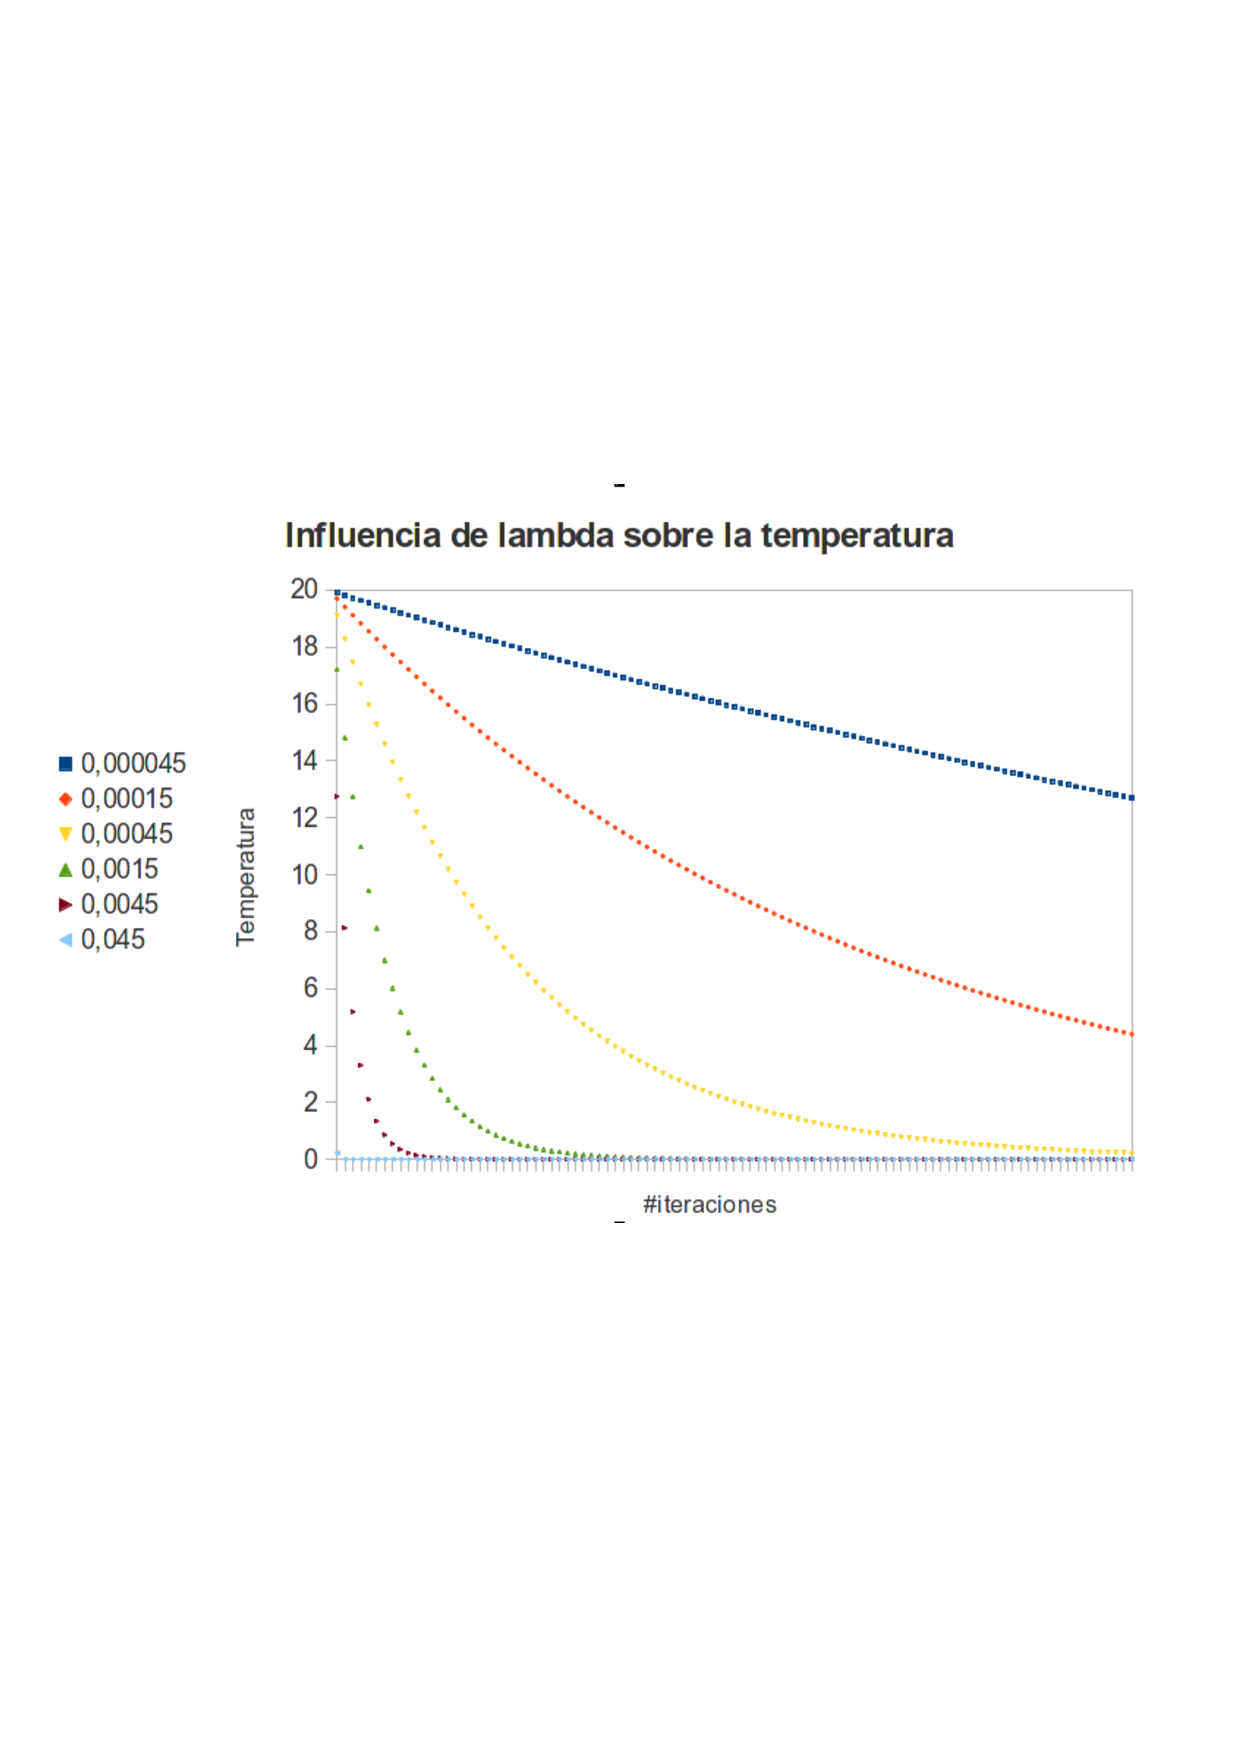
\includegraphics[width=12cm]{cordero}\\
{\it Fig. 2.1 : Influencia de $\lambda$ sobre la temperatura.}
\end{center}

Guardamos los valores por defecto $L=100$ y $K=20$ ; $N_{it} = 10 000$.
Se nota que el tiempo de ejecución no varia significativamente (~700ms), asi que
no muestraremos su valor para el resto de los experimentos.\\

\begin{center}
\begin{tabular}{|l||l|l|l|}
\hline
$\lambda$ & Estados mejorados & Beneficio & Mejoría\\
\hline
0.000045 & 41 & 98185 & 0,869\%\\
\hline
0,00045 & 40 & 98223 & 0,915\%\\
\hline
0,0045 & 39 & 98148 & 0,833\%\\
\hline
0,045 & 39 & 98123 & 0,800\%\\
\hline
0,45 & 30 & 97908 & 0,575\%\\
\hline\\
\end{tabular}
{\it Tabla 2.5 : Influencia de $\lambda$.}
\end{center}

El valor de lambda debe ser suficiente para tener una funcion de temperatura que
converga en 10 000 iteraciones, pero bastante pequeno para que no converga
demasiado rapido.

Escogemos $\lambda = 0,00045$ para el resto de experimentos.\\

\textbf{Influencia de $L$ : }

La constante $L$ representa la granularidad de la función de temperatura, es
decir el numero de iteraciones que se hacen entre cada canvio del valor de la
función. Podemos ver su efecto sobre el valor de $T$ en la figura Fig. 2.2 :
\begin{center}
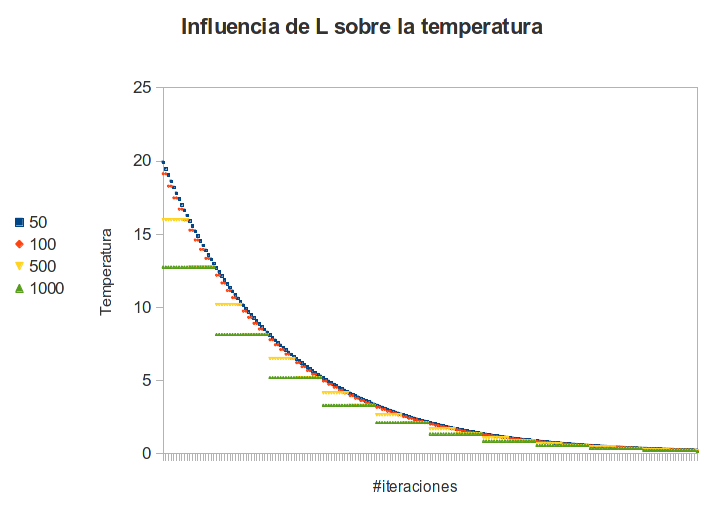
\includegraphics[width=12cm]{L}\\
{\it Fig. 2.2 : Influencia de $L$ sobre la temperatura.}
\end{center}

Guardamos el valor por defecto $K=20$ ; $N_{it} = 10 000$ y $\lambda = 0,00045$.

\begin{center}
\begin{tabular}{|l||l|l|l|}
\hline
$L$ & Estados mejorados & Beneficio & Mejoría\\
\hline
10 & 40 & 98172 & 0,857\%\\
\hline
100 & 40 & 98223 & 0,915\%\\
\hline
500 & 37 & 98044 & 0,721\%\\
\hline
1000 & 36 & 98140 & 0,820\%\\
\hline\\
\end{tabular}
{\it Tabla 2.6 : Influencia de $L$.}
\end{center}

Constatamos que una granularidad demasiado importante disminuye el porcentaje de
estados mejorados, pero una granularidad demasiado fina tambien impacta
negativamente el resultado del algoritmo.

Decidimos conservar el valor $L=100$ para el resto de experimentos.\\

\textbf{Influencia de $K$ : }

La constante $K$ representa l'amplituda de la función de temperatura.
Podemos ver su efecto sobre el valor de $T$ en la figura Fig. 2.3 :
\begin{center}
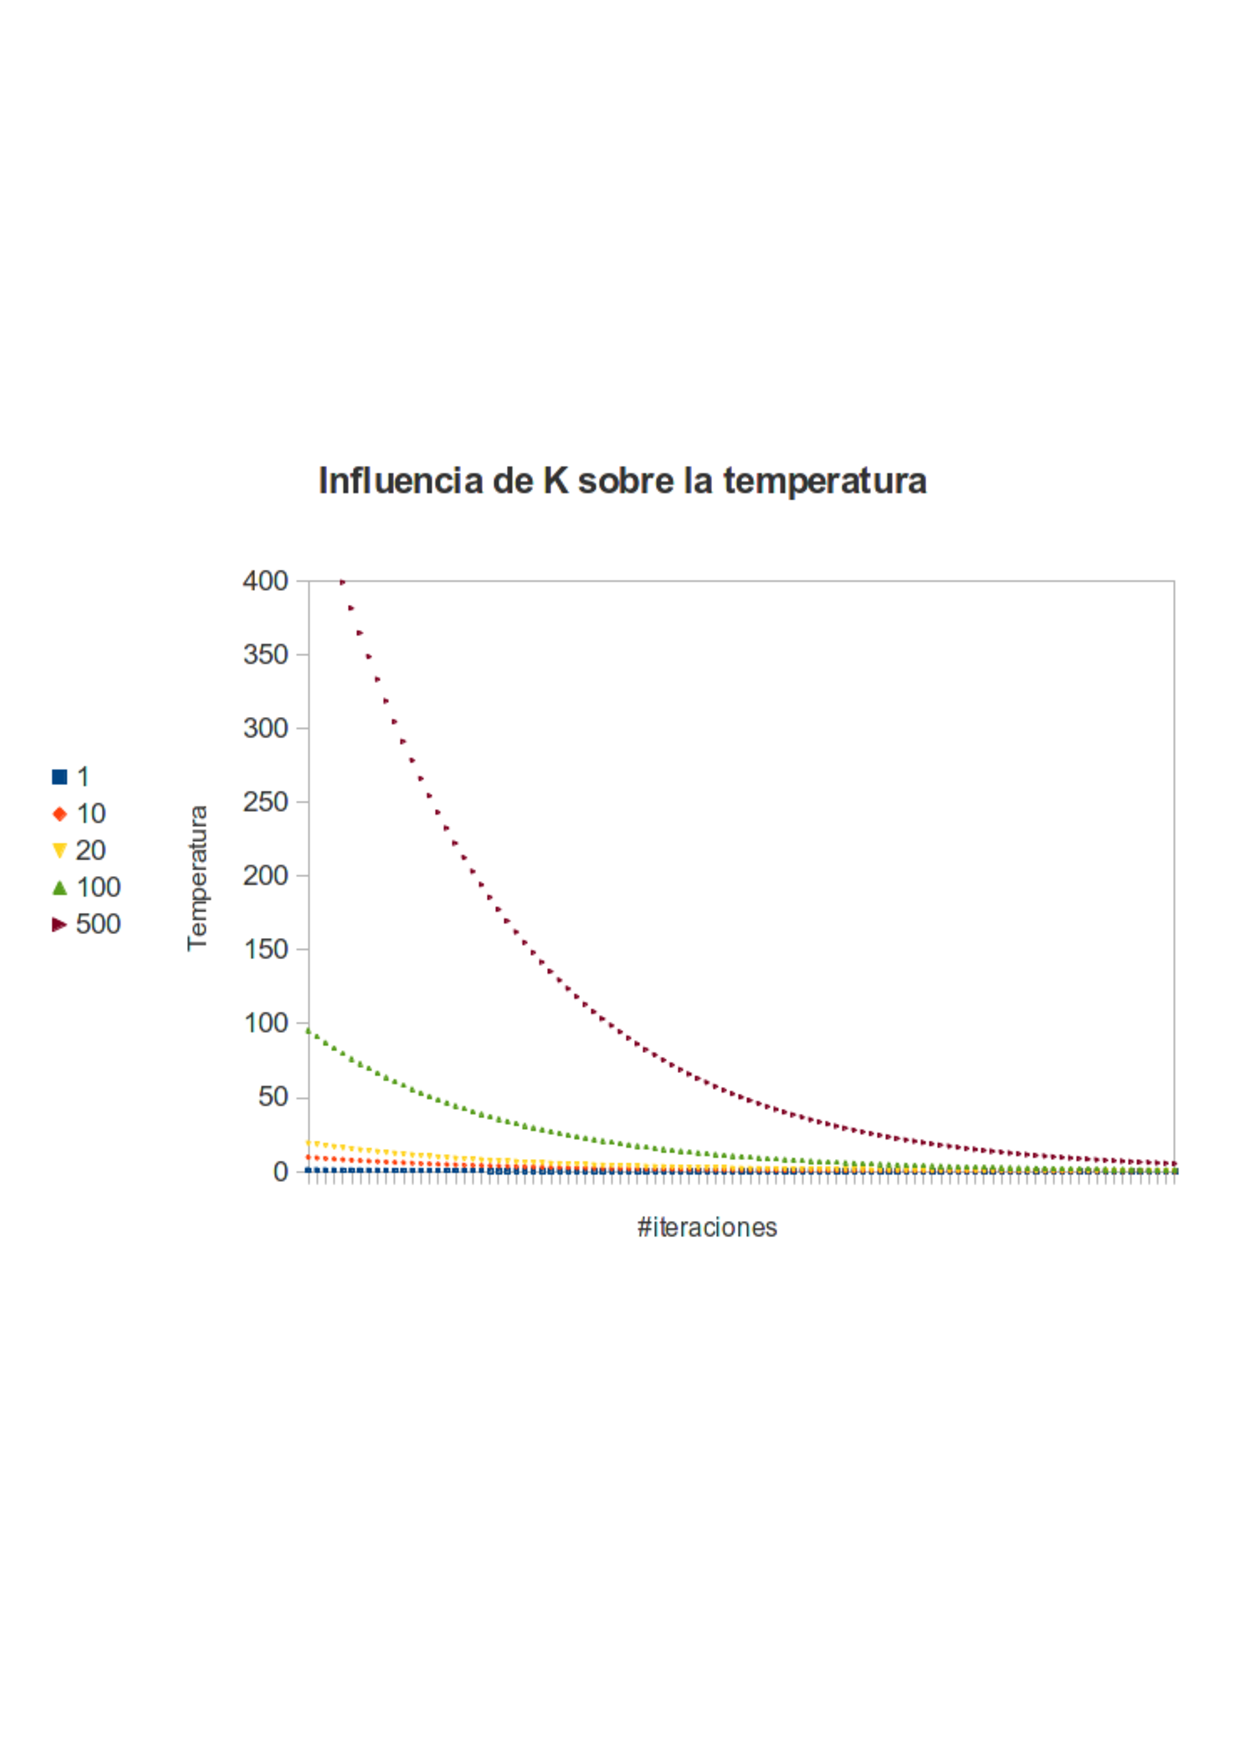
\includegraphics[width=12cm]{K}\\
{\it Fig. 2.3 : Influencia de $K$ sobre la temperatura.}
\end{center}

Ejecutamos las pruebas con los valores $N_{it} = 10 000$, $\lambda = 0,00045$ y
$L=100$.

\begin{center}
\begin{tabular}{|l||l|l|l|}
\hline
$K$ & Estados mejorados & Beneficio & Mejoría\\
\hline
1 & 38 & 98195 & 0,882\%\\
\hline
10 & 35 & 98134 & 0,813\%\\
\hline
20 & 40 & 98223 & 0,915\%\\
\hline
100 & 39 & 98067 & 0,760\%\\
\hline
500 & 11 & 97428 & 0,0764\%\\
\hline\\
\end{tabular}
{\it Tabla 2.7 : Influencia de $K$.}
\end{center}

$K$ es el factor que adapta la magnitud de la funcion de temperatura a la
cantidad a la cual se compara dentro del algoritmo del Simulated Annealing. Esta
cantidad es la diferencia entre los valores de la heuristica del estado y de su
sucesor. Decidimos conservar el valor $K=20$.

\subsubsection{Conclusiones}

Al ver el resultados de los tests, escogiremos como parámetros del Simulated
Annealing :
\begin{itemize}
\item 10 000 iteraciones
\item $\lambda = 0,00045$ para el coeficient de la exponencial
\item $L=100$ para la granularidad
\item $K=20$ para el coeficiente multiplicativo
\end{itemize}

\subsection{Experimento 4 : Influencia del numero de peticiones}

\subsubsection{Contexto}
\begin{description}
\item[Numero de pruebas :] 100 para cada numero de peticiones diferente.
\end{description}

\subsubsection{Resultados}

\begin{center}
\begin{tabular}{|l|l|l|l|l|l|}
\hline
\#peticiones & Tiempo de generación & \#iteraciones & Estados mejorados &
Beneficio (mejoria) & Tiempo total (por iteracion)\\
\hline
200 & 0,693ms & 2,16 & 24 & 94014 (0,297\%) & 74,02ms (35,78)\\
\hline
300 & 1,44ms & 1 & 0 & 69027 (0,00\%) & 25,14ms (25,14ms)\\
\hline
350 & 1,26ms & 1 & 0 & 35226 (0,00\%) & 27,30ms (27,30ms)\\
\hline
400 & 1,49ms & 1 & 0 & -584 (0,00\%) & 28,24ms (28,24ms)\\
\hline\\
\end{tabular}
{\it Tabla 2.8 : Resultados del experimento 4.}
\end{center}

\subsubsection{Conclusiones}
%TODO

\subsection{Experimento 5 : Influencia de la heurística}

\subsubsection{Contexto}
\begin{description}
\item[Numero de pruebas :] 100 para cada numero de peticiones y heuristica
diferente.
\end{description}

\subsubsection{Resultados}
con ret / con gan
200
n.it 6,88
ben 93850
mej 0,123
ret 58,67 / 71,9
mej 20,67 / 3,44
t 198,5/29,15

250
n.it 3,07
ben 97405
mej 0,0523
ret 747,5 / 754,1
mej 1,211 / 0,268
t 62,02/21,37

300
n.it 1,1
ben 69022
mej -0,00683
ret 2046,39 / 2046,16
mej 0,0113 / 0
t 26,60/24,56

\subsubsection{Conclusiones}
%TODO

\subsection{Experimento 6 : Comparación de los algoritmos}

\subsubsection{Contexto}
\begin{description}
\item[Numero de pruebas :] 100 para cada numero de peticiones y algoritmo
diferente.
\end{description}

\subsubsection{Resultados}
SA-gan
\begin{center}
\begin{tabular}{|l||l|l|l||l|l|l|}
\hline
\#peticiones & Estados mejorados & Beneficio & Mejoría & ret & Tiempo de
ejecucion\\
200 & 89 & 94445 & 0,748\% & 282 & -344\% & 526ms\\
\hline
250 & & & & & & \\
\hline
300 & 0 & 69027 & 0\% & 2046 & 0\% & 836ms\\
\hline
\end{tabular}
{\it Tabla}
\end{center}
SA-ret
\begin{center}
\begin{tabular}{|l||l|l|l||l|l|l|}
\hline
\#peticiones & Estados mejorados & Beneficio & Mejoría & ret & Tiempo de
ejecucion\\
\hline
200 & 7 & 93442 & -0,310\% & 74,75 & 1,07\% & 628ms\\
\hline
250 & 83 & 70853 & -27,3\% & 664 & 11,2\% & 711ms\\
\hline
300 & 100 & 16909 & -76,4\% & 1431 & 30,0\% & 854ms\\
\hline
\end{tabular}
{\it Tabla}
\end{center}

retrso > baja del beneficio


\subsubsection{Conclusiones}

\subsection{Experimento 7 : Influencia de la repartición de capacidades
de los camiones}

\subsubsection{Contexto}
100

\subsubsection{Resultados}

1 : 30 15 15
t. gen init : 1,95
n.it : 1
ben 62989
ret 1517
t 30,05

2 : 15 30 15
gen 1,73
n.it : 1
ben 90560
ret 929
t 28,16

3 : 15 15 30
gen 0,484
n it : 5,3
57\% de mejora
ben : 115851 (1,16)
ret 147 (14,5)
t 218,7 (44,74)

\subsubsection{Conclusiones}

\subsection{Experimento 8 : Influencia de la distribución de probabilidad
de horas de entregas}

\subsubsection{Contexto}
100

\subsubsection{Resultados}

todo junto :
t gen 1,00
n it 1,15
ben 97201 (0.135)
ret 768 (0,299)
t g 32,10 (26,49)

1era 4 :
t gen 1,19
n it 1,09
mej 3
ben 97298 (0,0726)
ret 759 (0,213)
t 32,66 (29,42)

untimas 4
t gen 0,94
n it 1,28
mej 8
ben 97673 (0,234)
746 (0,63)
33,46 (25,27)

2 1os 2 ult
t gen 0,819
n it 1,32
mej 11
ben 97547 (0,313)
ret 741 (0,653)
41,53 (32,34)

8 11 14 17
0,911
1,08
mej 3
ben 96740 (0,0787)
ret 779 (0,166)
32,98 (27,67)

8 12 13 17
0,832
1,12
4
97625 (0,108)
769 (0,195)
30,05 (25,91)

\subsubsection{Conclusiones}

\section*{Conclusión}

\end{document}
